\section{Experimentos}

Ao final da etapa de previsões foi gerada uma imagem para cada indicador contendo os 
valores previstos para o período de teste, bem como os valores reais referentes aos 
períodos de treinamento, validação e teste, vide as figuras 1, 2 e 3.  Como extensão 
dessa etapa, o modelo também foi avaliado de acordo com as métricas de avaliação 
definidas pela metodologia do estudo, vide as tabelas 3, 4, 5.

\begin{figure}[h!]
    \centering
    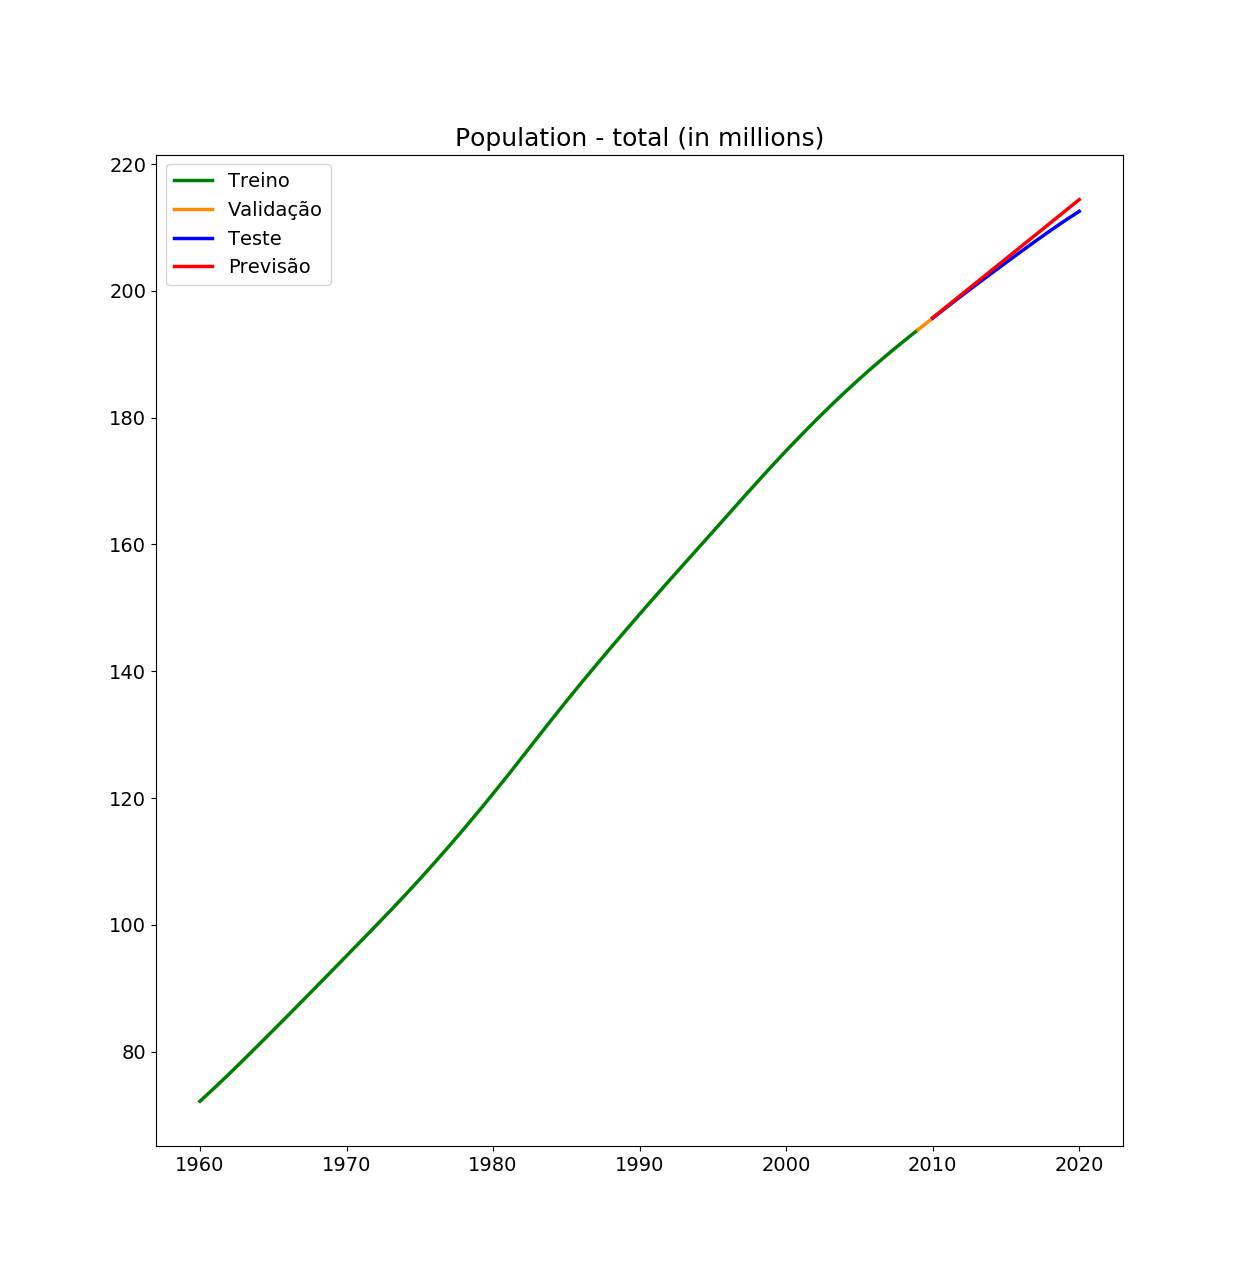
\includegraphics[scale=0.35]{images/Figure_1}
    \caption{Modelagem da previsão para o indicador “SP.POP.TOTL”}
\end{figure}

Na figura 3 é apresentada a modelagem da previsão para o indicador “SP.POP.TOTL”, que apresenta a população 
brasileira ao longo dos anos, em milhões de pessoas. A tabela 3 apresenta os valores 
obtidos para as métricas de avaliação do modelo. A partir do exposto, é possível ver como a 
modelagem performou dentro do objetivo estabelecido nas duas métricas, e apresentou um desvio negligenciável.


\begin{table}[h!]
    \centering
    \begin{tabular}{|c|c|}
        \hline
        \multicolumn{1}{|p{5cm}|}{Métrica de avaliação para a previsão de "\emph{Population - total (in millions)}"} & Valor \\
        \hline 
        \emph{MAE Score} & 0.7305939401983349 \\
        \hline
        \emph{R2 Score} &  0.9703244706047911 \\
        \hline
    \end{tabular}
    \caption{Avaliação da performance do modelo no conjunto de teste com as métricas \emph{MAE} e \emph{R2}}
\end{table}

\begin{figure}[h!]
    \centering
    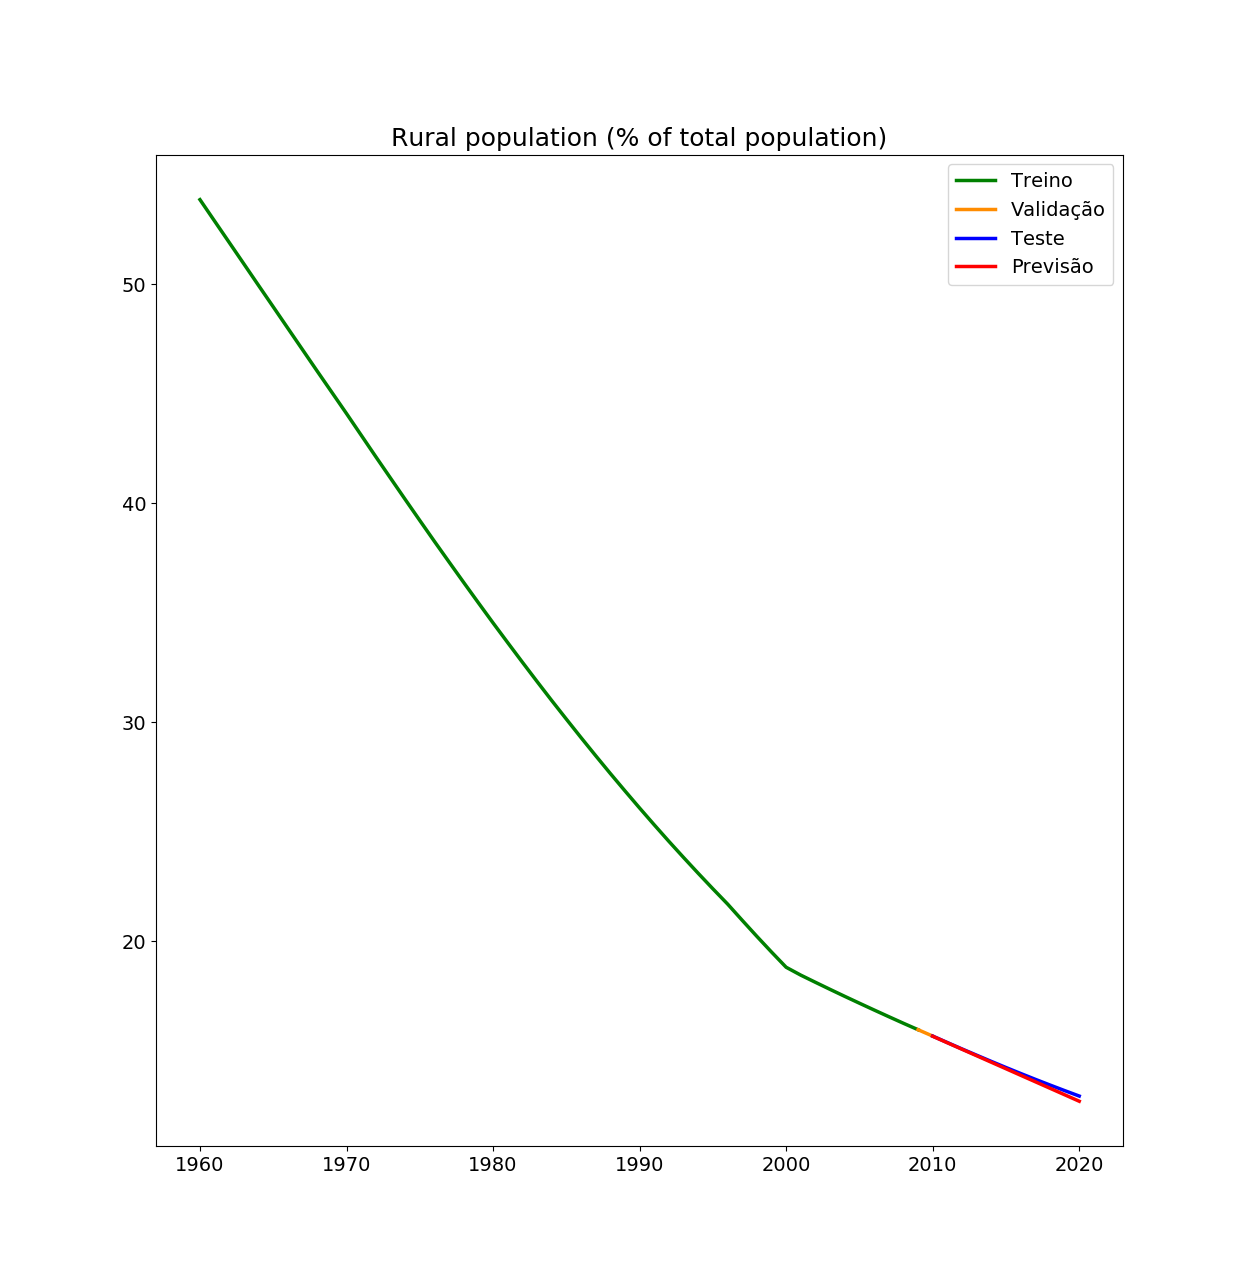
\includegraphics[scale=0.35]{images/Figure_2}
    \caption{Modelagem da previsão para o indicador ``SP.RUR.TOTL.ZS''}
\end{figure}

Na figura 4 é vista a modelagem da previsão para o indicador ``SP.RUR.TOTL.ZS'', 
que apresenta a porcentagem da população brasileira que vive em áreas rurais ao longo dos anos. 
A tabela 4 apresenta os valores obtidos para as métricas de avaliação do modelo em relação a esse indicador.

\begin{table}[h!]
    \centering
    \begin{tabular}{|c|c|}
        \hline
        \multicolumn{1}{|p{5cm}|}{Métrica de avaliação para a previsão de \emph{"Rural population (\% of total population)"}} & Valor \\
        \hline
        \emph{MAE Score} & 0.0829616118683835 \\
        \hline
        \emph{R2 Score} & 0.9832934099951631 \\
        \hline 
    \end{tabular}
    \caption{Avaliação da performance do modelo no conjunto de teste com as métricas \emph{MAE} e \emph{R2}}
\end{table}

\begin{figure}[h!]
    \centering
    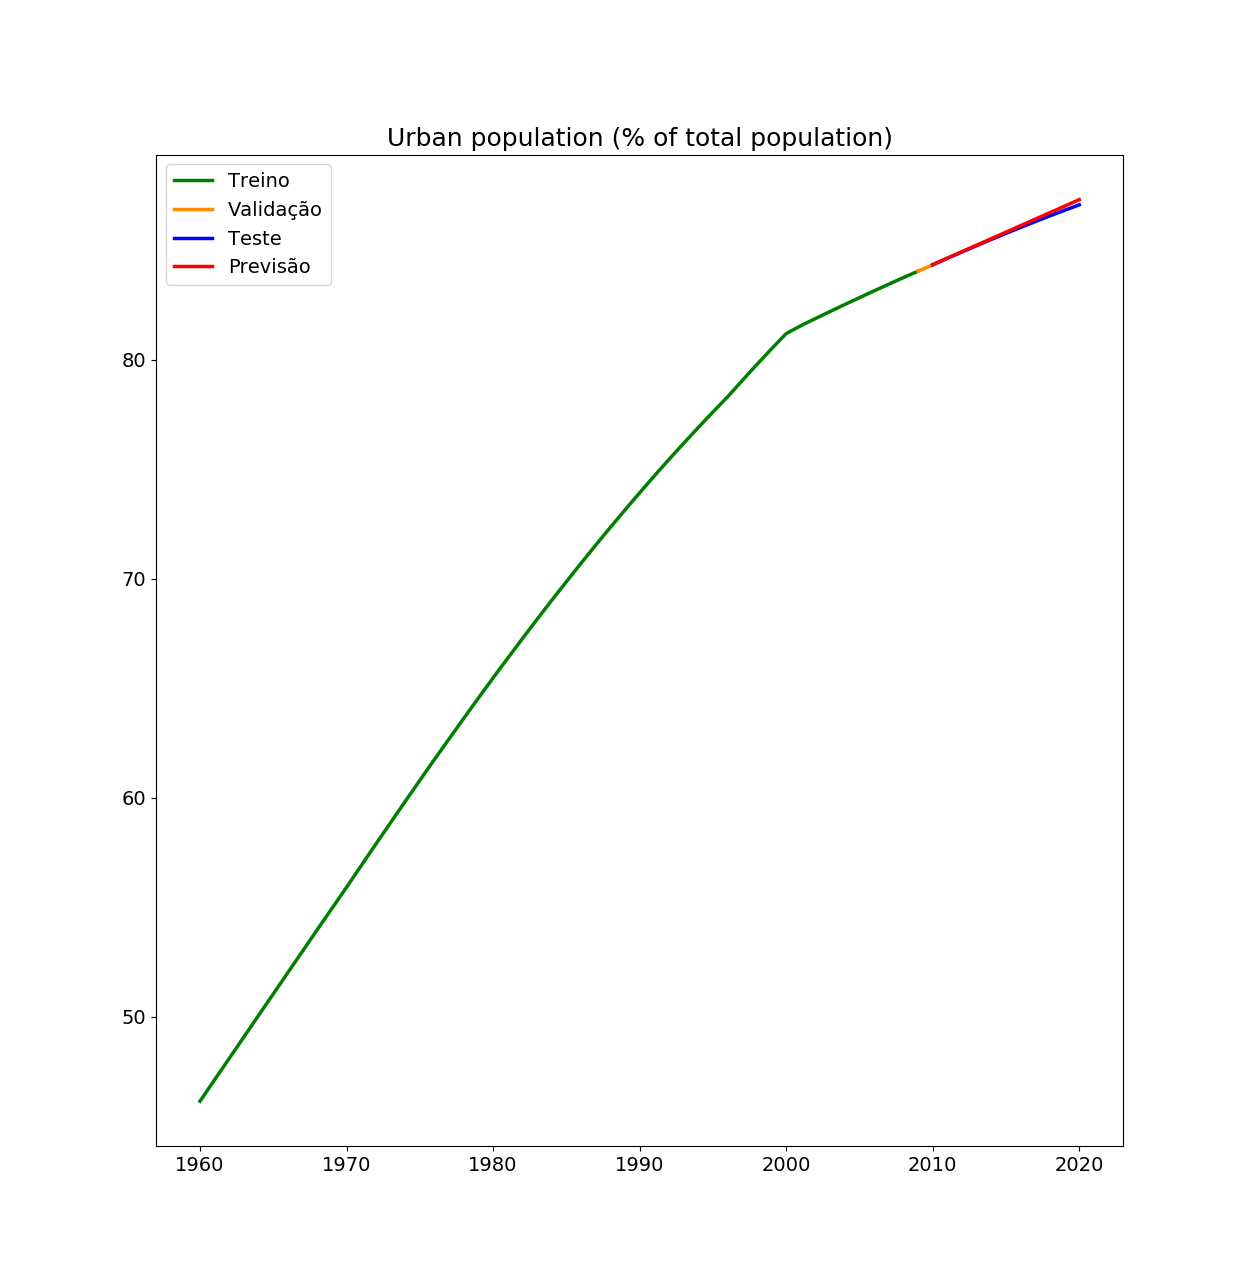
\includegraphics[scale=0.35]{images/Figure_3}
    \caption{Modelagem da previsão para o indicador “SP.URB.TOTL.IN.ZS”}
\end{figure}

Na figura 5 é vista a modelagem da previsão para o indicador ``SP.URB.TOTL.IN.ZS'', que apresenta a porcentagem 
da população brasileira que vive em centros urbanos ao longo dos anos. A tabela 5 apresenta os valores 
obtidos para as métricas de avaliação do modelo em relação a esse indicador. 

\begin{table}[h!]
    \centering
    \begin{tabular}{|c|c|}
        \hline
        \multicolumn{1}{|p{5cm}|}{Métrica de avaliação para a previsão de Urban population ``(\emph{\% of total population})"} & Valor \\
        \hline
        \emph{MAE Score} & 0.08296161186839222 \\
        \hline 
        \emph{R2 Score} & 0.9832934099951601 \\
        \hline
    \end{tabular}
    \caption{Avaliação da performance do modelo no conjunto de teste com as métricas \emph{MAE} e \emph{R2}}    
\end{table}